Figure~\ref{fig:MitM-graph} shows an overview of the MitM ontology, together with the
system APIs and the alignments (in red). We can directly see that the MitM ontology is
dwarfed by the system API graphs. This is to be expected, since we have mainly covered the
background knowledge needed for the OpenDreamKit integration use cases;
see~\cite{ODK-D6.5}. This is in sync with the overall project plan, which mainly wants to
demonstrate the feasibility of the MitM approach to system integration, and expects the
main part of the MitM Ontology to be contributed by the mathematical community.

Most of the work in MitM Ontology has gone into provisioning a viable foundation
and basic set of types, which allow the flexiformalization and specification of
mathematical knowledge, objects, functions, and types in a system-independent/neutral way
that closely mirrors the presentation in the mathematical literature. The central focus
was in the naturalness and adequacy of the representation. The focus on a basic repertoire
of types inspired by mathematical practice goes a long way into this direction.

With CGT (computational group theory) we have shown that the MitM approach is feasible,
and that the investment into the extension of the MitM Ontology is commensurate with
writing good (mathematical) documentation. Indeed the MitM ontology together with the
system API alignments can be used for documentation purposes and complement it. Moreover, as
MitM representations are shared between systems by design, all systems participating in
the OpenDreamKit MitM-based integration scheme obtain this ``documentation'' for the cost
of alignments alone. 

Generally, we note that the investment necessary for adding mathematical functionality to
the MitM integration decreases with the size of the existing MitM ontology, and in the
limit becomes proportional to the size of the added functionality, while the amount of
system functionality yielded by MitM-compatible systems increases proportionally with the
MitM size. Already with four systems GAP, Sage, Singular, and LMFDB; see~\cite{ODK-D6.5}
we have reached a size where investments into extending the MitM ontology are starting to
pay off, and interest of the computational mathematics is generated. We expect that, once
the heavy lifting of getting the framework and a seed MitM Ontology has been done,
the integration framework and MitM Ontology coverage will grow organically.

\begin{figure}\centering
  \fbox{\begin{sideways}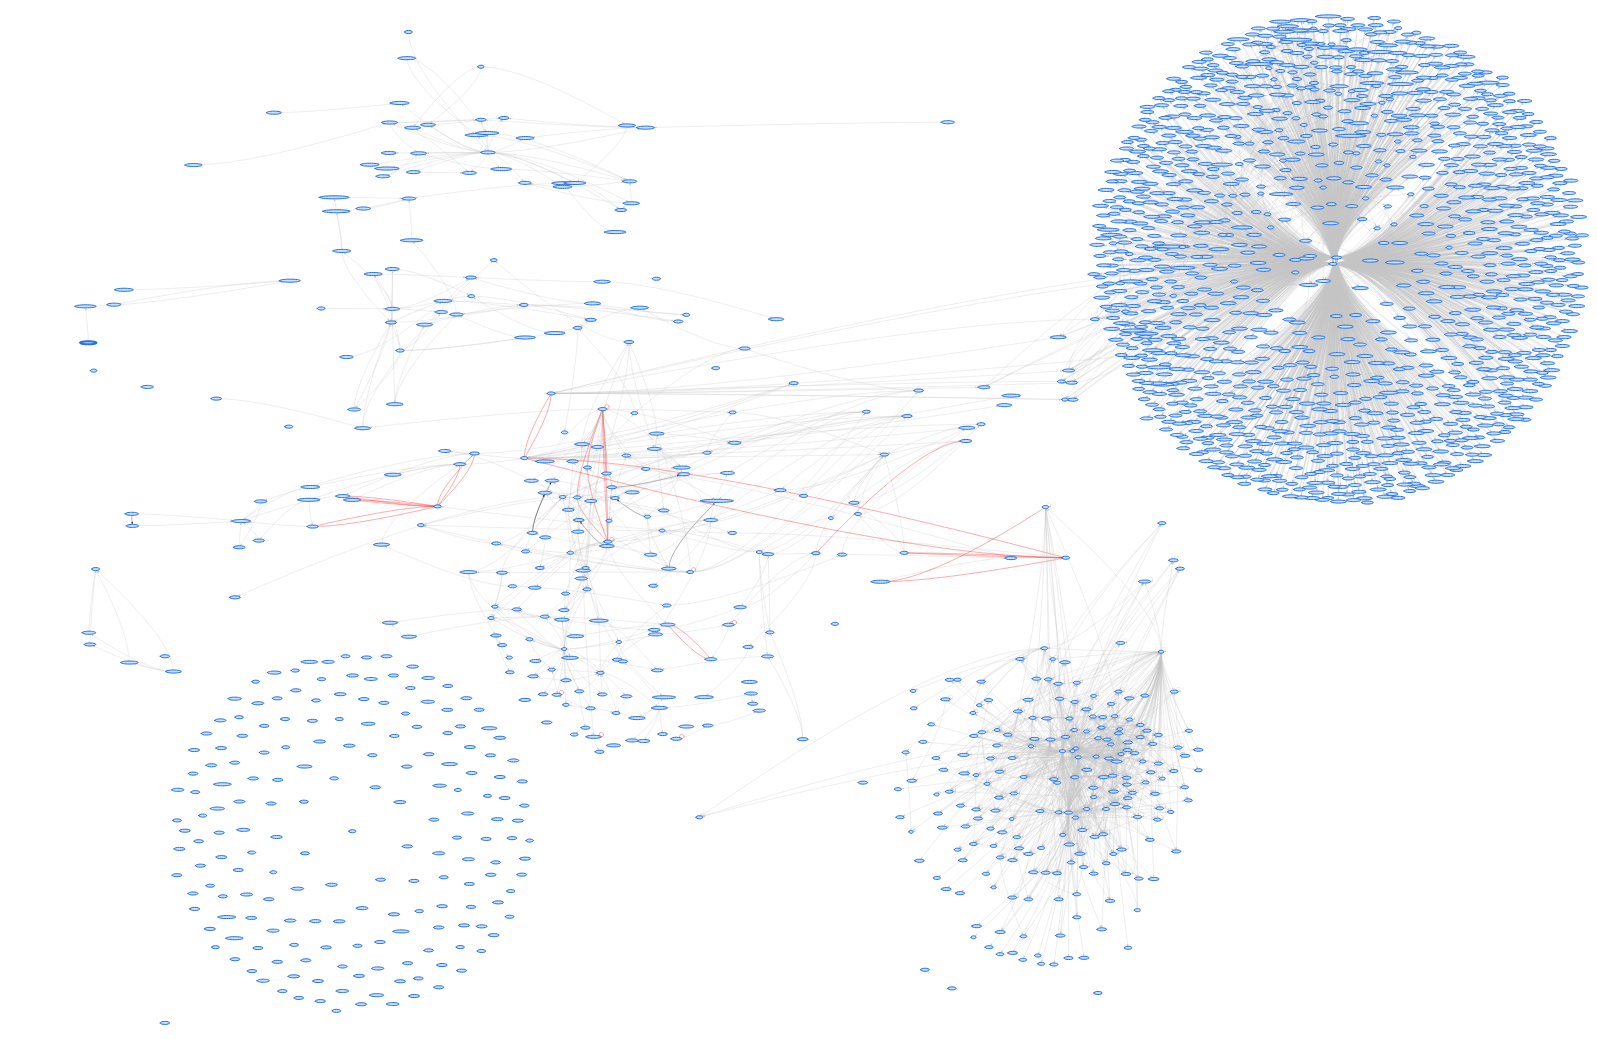
\includegraphics[width=.95\textheight]{MitM-graph}\end{sideways}}
%  \fbox{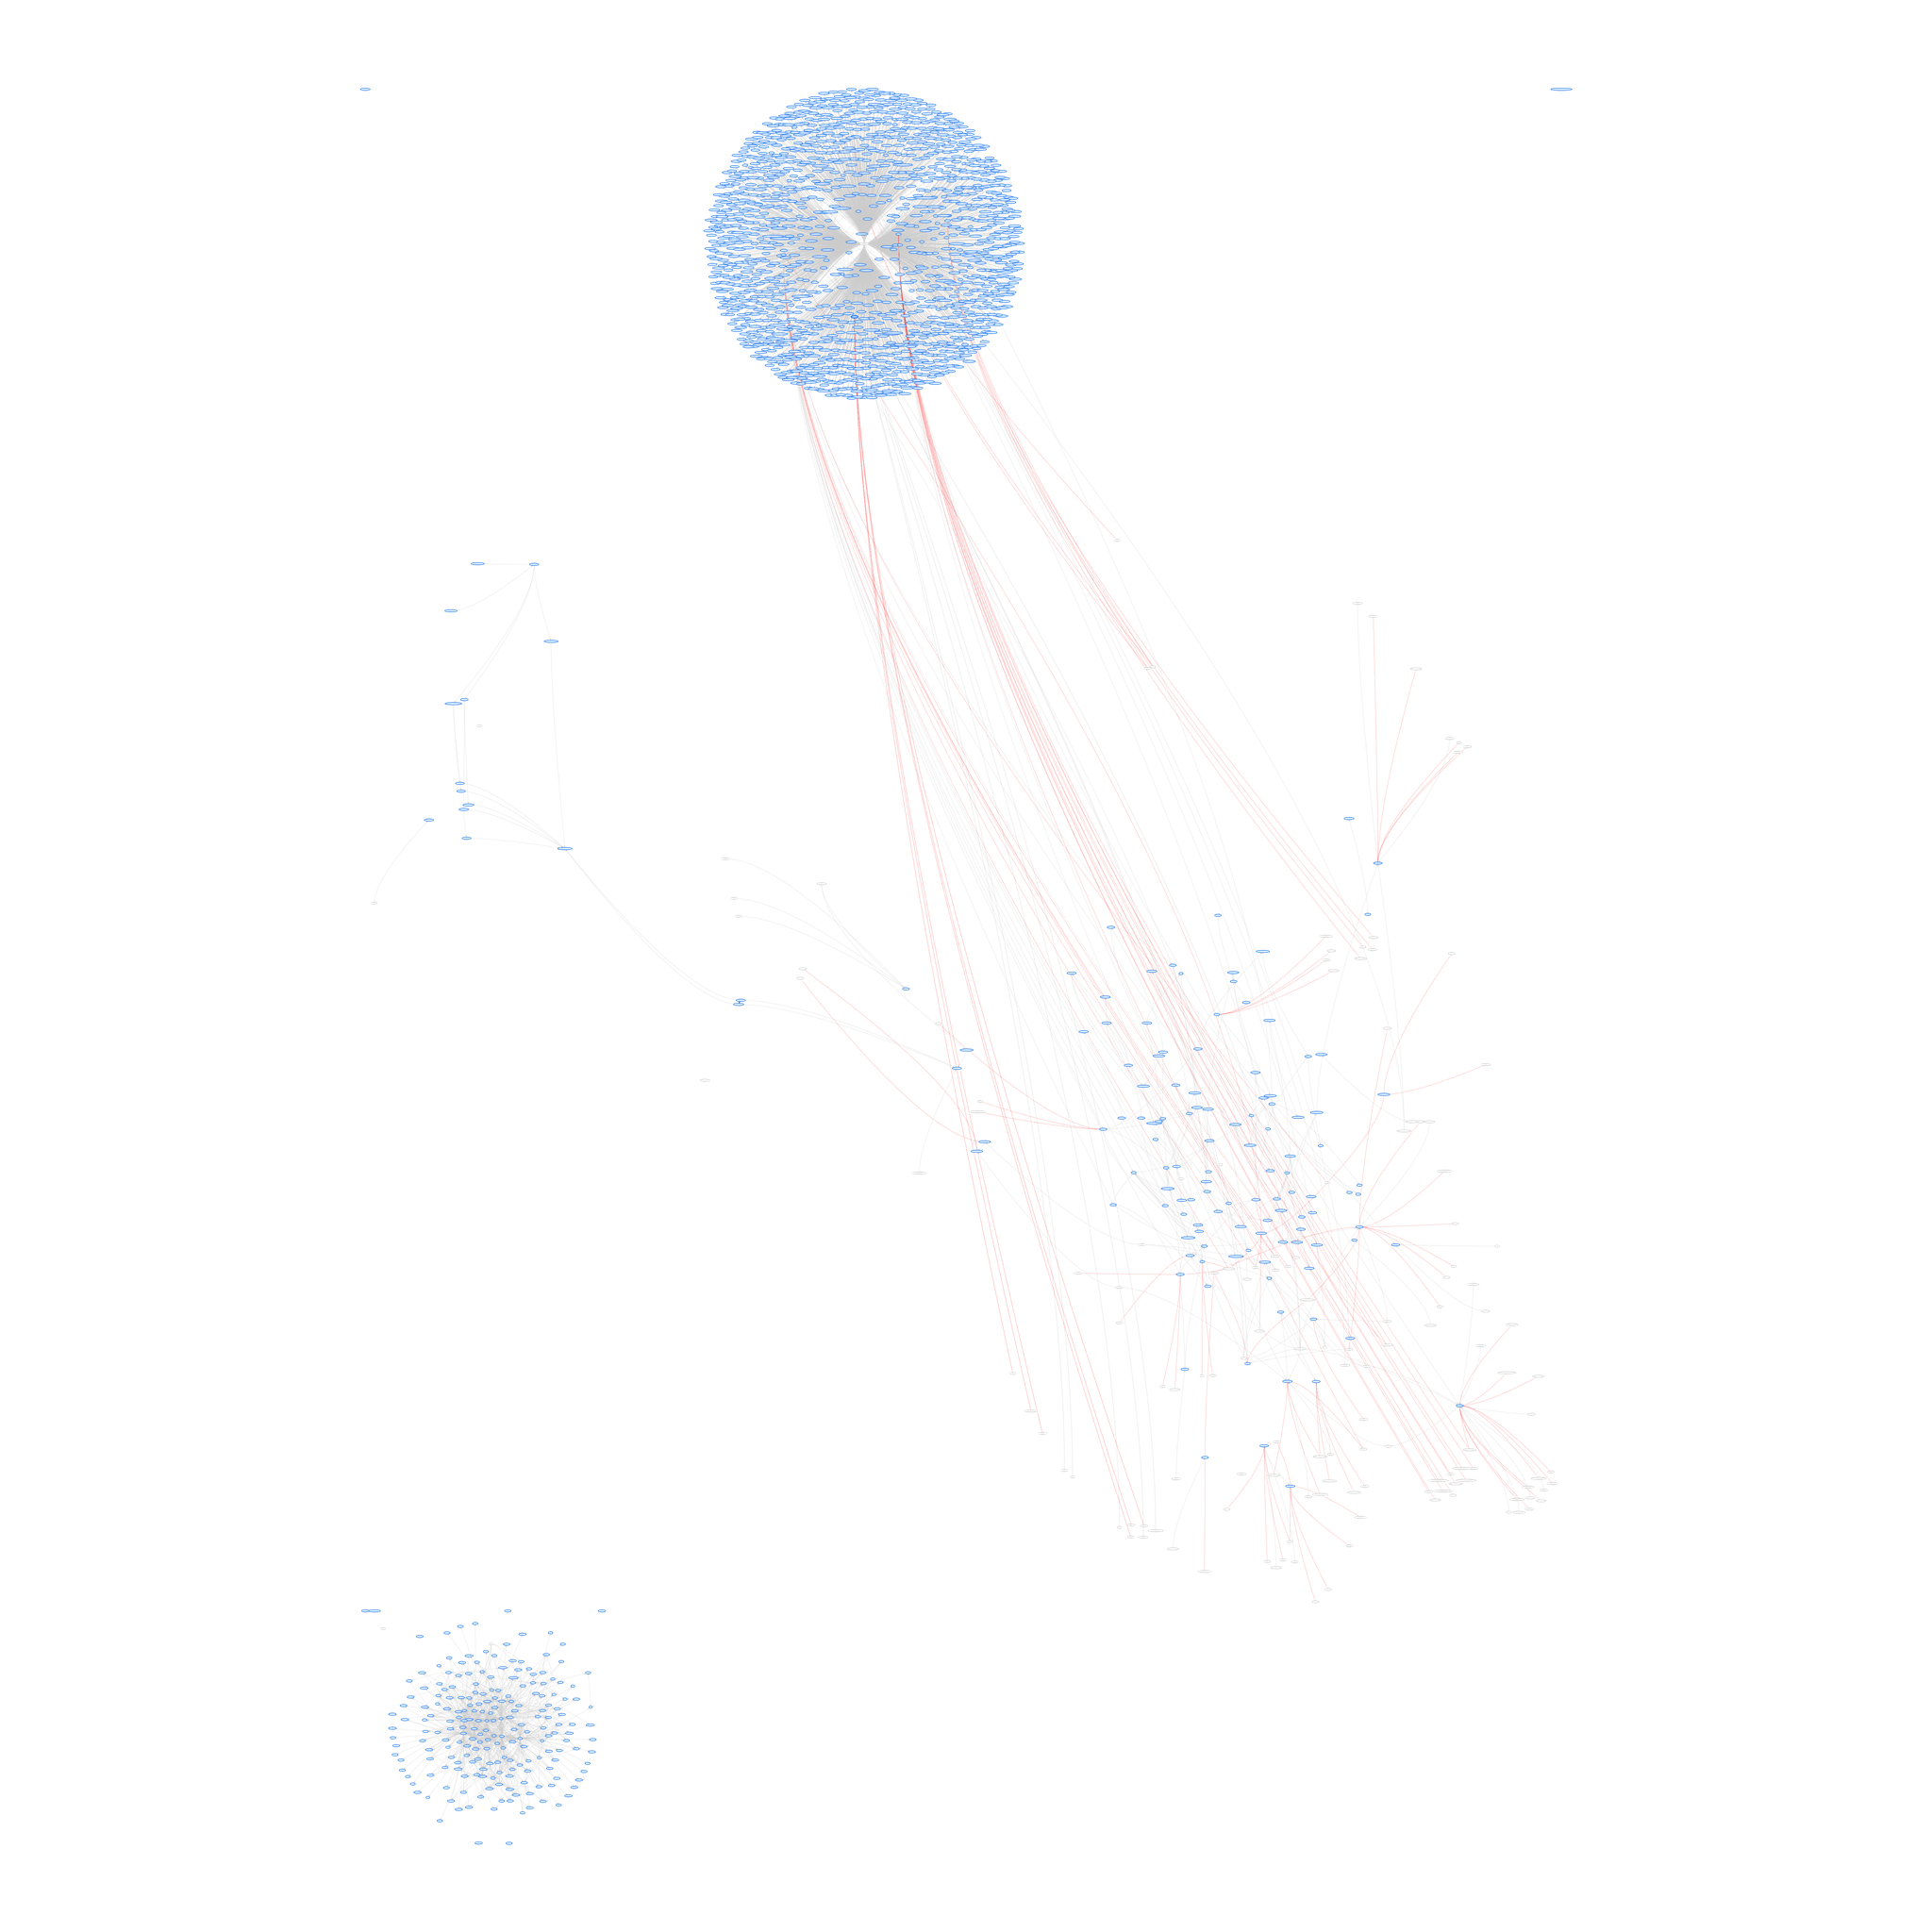
\includegraphics[width=.95\textwidth]{MitM-graph1}}
  \caption{The MitM Theory Graph}\label{fig:MitM-graph}
\end{figure}

%%% Local Variables:
%%% mode: visual-line
%%% fill-column: 5000
%%% mode: latex
%%% TeX-master: "report"
%%% End:

%  LocalWords:  fig:MitM-graph flexiformalization MitM-based centering fbox textheight
%  LocalWords:  includegraphics MitM-graph textwidth MitM-graph1
